\documentclass[aps,prapplied,reprint,amsmath,amssymb,floatfix]{revtex4-2}
% If revtex4-2 is unavailable, switch the first line to:
%   \documentclass[twocolumn]{article}
% and delete the \affiliation lines below.
\usepackage{graphicx}
\usepackage{booktabs}
\usepackage{bm}
\usepackage{xcolor}

\begin{document}

\title{Breaking point-group symmetry activates even-order computation\\
in modal physical reservoirs}

\author{Gavin Branaa}
\affiliation{Independent Researcher}

\date{\today}

\begin{abstract}
Physical reservoir computing exploits the nonlinear dynamics of a fixed
material substrate, training only a linear readout. A widespread intuition
holds that geometrically ``richer'' substrates---quasicrystalline or otherwise
aperiodic resonator structures---should make better reservoirs. Using a
finite-element modal model of a perforated micro-plate, we find that this
intuition is largely false: the structural richness of a quasicrystalline mode
spectrum, and of the mode-shape-determined nonlinear coupling network, is real
but \emph{computationally inert}. The one genuine advantage we identify has a
different origin and an exact explanation. We prove a point-group
\emph{selection rule}: on a substrate with the square's $D_4$ symmetry, the
integral $\int \phi_i^3\,dA$---the modal strength of the even-order
nonlinearity that alone can generate products of past inputs---vanishes
identically for every mode except those of the totally symmetric representation
$A_1$, forcing a fraction $7/8$ of modes to be ``product-blind.'' Breaking the
point symmetry lifts the prohibition. The consequence is a statistically robust
but sharply bounded computing benefit: on shallow even-order tasks in the
weakly coupled regime, a symmetry-broken substrate outperforms a symmetric one
(paired $p\!\sim\!10^{-13}$, surviving cross-validation and feature
standardization), with the advantage scaling monotonically with the degree of
symmetry breaking. A \emph{periodic} but low-symmetry substrate captures about
half the effect; a quasicrystal, the maximal symmetry breaker, captures the
most. We argue the operative design principle is symmetry breaking, not
aperiodicity, and that it applies to any modal physical computer.
\end{abstract}

\maketitle

\section{Introduction}

Physical reservoir computing offloads the costly nonlinear transformation of a
learning task onto the intrinsic dynamics of a physical system---a network of
oscillators, a photonic cavity, a spintronic film, a vibrating
plate---while training only a linear output map~\cite{jaeger2001,maass2002,tanaka2019}. Its appeal
is hardware efficiency: if the substrate already performs a high-dimensional,
fading-memory, nonlinear embedding of the input, computation becomes almost
free. This raises an obvious design question: \emph{what makes a good physical
substrate?}

A recurring intuition is that geometric or spectral ``richness'' helps.
Quasicrystalline and other aperiodic resonator geometries, with their dense,
non-degenerate mode spectra and spatially intricate eigenmodes, are natural
candidates for ``richer'' reservoirs. Here we test that intuition directly in
a controlled finite-element model and find it wanting. The richness of a
quasicrystalline substrate is genuinely present---its spectrum has far fewer
near-degenerate modes than a periodic counterpart, and its mode-shape-derived
nonlinear coupling network is markedly denser---yet neither property confers
any measurable reservoir-computing advantage.

The single robust advantage we do find is unrelated to richness. It is a
consequence of \emph{symmetry}, and it admits an exact, group-theoretic proof.
The even-order (product-generating) nonlinearity of a mode is controlled by the
overlap integral $\int\phi_i^3\,dA$; on a substrate with the square point
group $D_4$ this integral is forced to zero for all but the totally symmetric
modes. Breaking the symmetry activates the even-order nonlinearity in every
mode. The resulting computing benefit is real and statistically clean but
narrow---confined to shallow even-order tasks in a weakly coupled regime---and,
crucially, is governed by how much symmetry is broken rather than by
aperiodicity per se. We make this precise below.

\section{Modal reservoir model}

We model a thin, fully clamped, square micro-plate of side
$L=100~\mu$m and thickness $h=100$~nm, with material constants $E=170$~GPa,
$\nu=0.28$, $\rho=2330~\mathrm{kg\,m^{-3}}$ (silicon-like). The plate is
perforated; perforation is represented by area-fraction homogenization of the
element stiffness and mass, avoiding mesh fragmentation. A Mindlin
shear-deformable quadrilateral finite-element discretization yields the
generalized eigenproblem $\bm{K}\bm\psi=\omega^2\bm{M}\bm\psi$, whose first
$N=40$ transverse modes $\phi_i(x,y)$ and frequencies $\omega_i$ define the
reservoir. Each mode shape is normalized to unit root-mean-square amplitude
over the plate, so that the two substrates we compare differ only in mode
\emph{shape and spacing}, not in overall scale.

We endow the plate with a pointwise transverse nonlinearity
$g(w)=a\,w^2+b\,w^3$ and project it onto the modal basis,
$w(x,y,t)=\sum_j x_j(t)\,\phi_j(x,y)$, giving the reduced dynamics
\begin{align}
\ddot x_i + 2\zeta\omega_i \dot x_i + \omega_i^2 x_i
&= -a\!\sum_{j,k} T_{ijk}\,x_j x_k
   -b\!\sum_{j,k,l} Q_{ijkl}\,x_j x_k x_l \nonumber\\
&\quad + \phi_i(\bm r_d)\,u(t),
\label{eq:modal}
\end{align}
with the geometry-determined coupling tensors
\begin{equation}
T_{ijk}=\!\int\!\phi_i\phi_j\phi_k\,dA,\qquad
Q_{ijkl}=\!\int\!\phi_i\phi_j\phi_k\phi_l\,dA .
\label{eq:tensors}
\end{equation}
The drive is a point actuator at $\bm r_d$, so the input couples to mode $i$
through $\phi_i(\bm r_d)$. We integrate Eq.~\eqref{eq:modal} with a
semi-implicit Euler scheme and read out a ridge-regularized linear combination
of the instantaneous features $\{x_i,\dot x_i,1\}$. A coupling-strength knob
$\gamma\in[0,1]$ interpolates between the fully coupled model ($\gamma=1$) and
an \emph{uncoupled} bank of independent nonlinear oscillators ($\gamma=0$), the
latter retaining only the self-terms $c^{(2)}_i\equiv T_{iii}=\int\phi_i^3\,dA$
and $c^{(3)}_i\equiv Q_{iiii}=\int\phi_i^4\,dA$.

We compare three substrates at matched $85\%$ hole coverage: a periodic
$9\times 9$ hole array with full $D_4$ symmetry; an eightfold de Bruijn
quasicrystalline array; and a low-symmetry \emph{periodic} array (a sheared,
anisotropic grid) that is regular but breaks $D_4$.

We benchmark with two standard probes. The \emph{product task}
$y[n]=u[n-1]\,u[n-2]$ is the minimal task that provably requires both memory
and nonlinearity; a linear reservoir cannot perform it. The
\emph{NARMA-10} system,
$y[n{+}1]=0.3\,y[n]+0.05\,y[n]\!\sum_{i=0}^{9}y[n{-}i]+1.5\,u[n]u[n{-}9]+0.1$,
is the field-standard recurrent benchmark.

\section{Structural richness is computationally inert}

We first confirm that the substrate's much-cited structural richness does not
help. The quasicrystalline spectrum has far fewer near-degenerate mode pairs
than the periodic one ($3$ vs.\ $18$), and its mode-shape-derived cubic
coupling network is $2.4\times$ denser (fraction of non-negligible triple
overlaps $T_{ijk}$: $0.84$ vs.\ $0.34$). Neither translates into performance.
On the product task and on short-term memory capacity, the two substrates tie
within seed-to-seed scatter at every reservoir size $N=6\ldots40$ and at every
coupling strength $\gamma$. Increasing $\gamma$ \emph{reduces} performance and
memory in both cases (Fig.~\ref{fig:saturation}); the dense quasicrystalline
coupling network confers no advantage at any operating point. The reservoir
needs only to be ``rich enough,'' a bar the periodic substrate already clears,
consistent with the broad observation that disparate reservoir topologies
perform comparably once sufficiently expressive~\cite{appeltant2011}.

\begin{figure}[t]
\centering
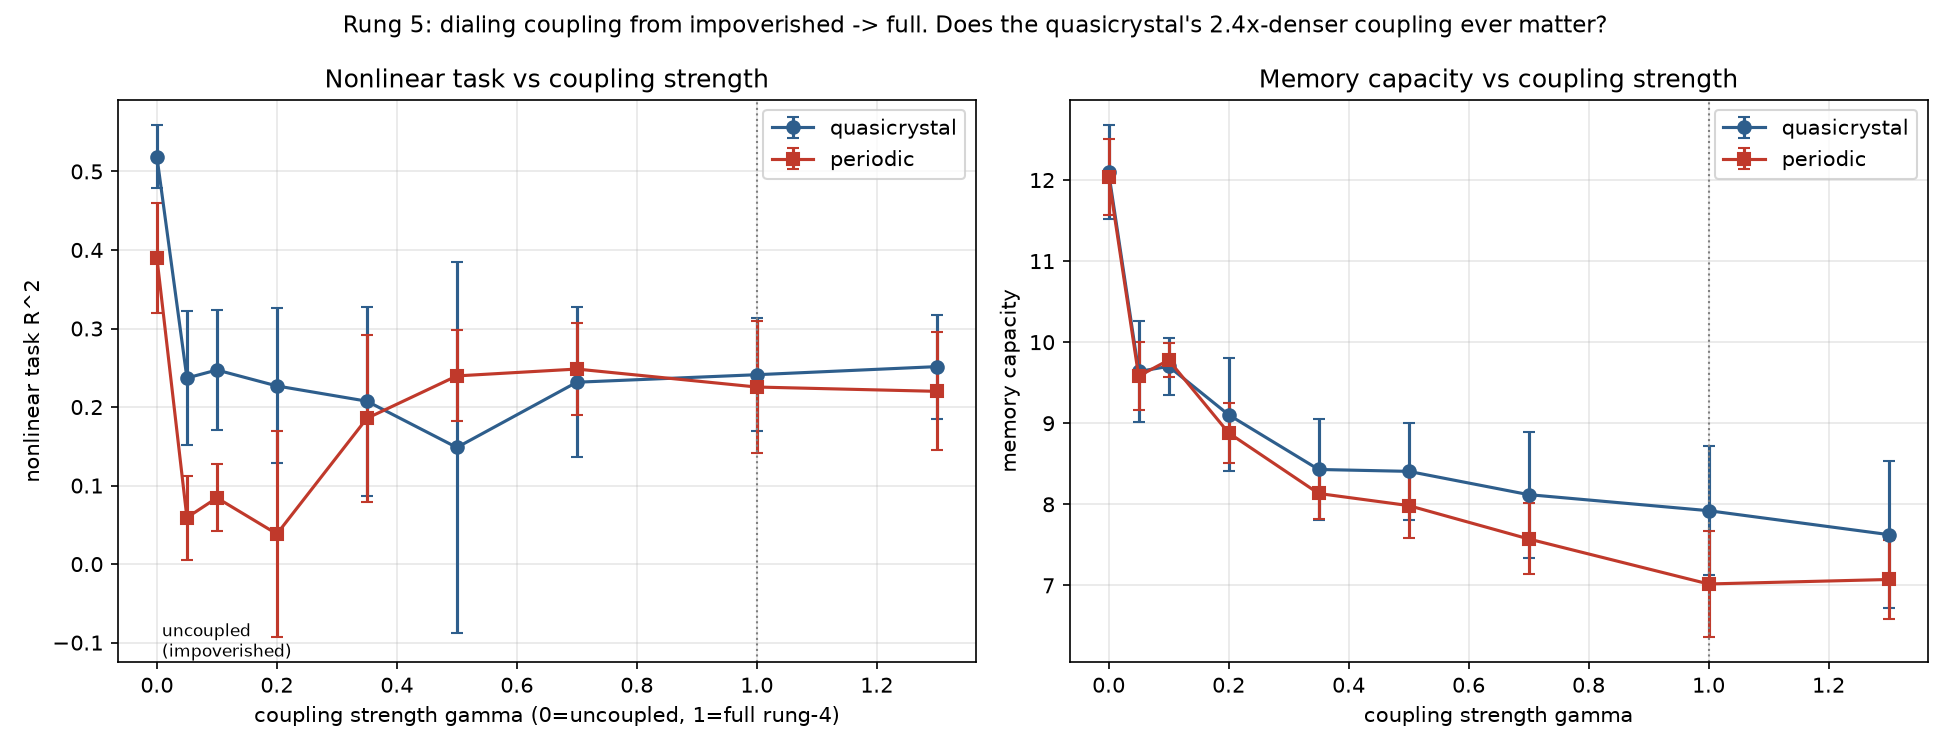
\includegraphics[width=\columnwidth]{reservoir_rung5_saturation.png}
\caption{Dialing inter-mode coupling from an uncoupled bank ($\gamma=0$) to
full strength. The quasicrystalline and periodic substrates track each other
on the product task and on memory capacity at all coupling strengths; the
$2.4\times$-denser quasicrystalline coupling network is inert. Performance is
highest uncoupled, where the per-mode even-order advantage of
Sec.~\ref{sec:rule} resides.}
\label{fig:saturation}
\end{figure}

\section{A point-group selection rule}
\label{sec:rule}

The only term in Eq.~\eqref{eq:modal} that can generate a \emph{product} of
two distinct past inputs---and hence perform an even-order task---is the
quadratic one, whose per-mode strength is $c^{(2)}_i=\int\phi_i^3\,dA$. (A
purely cubic, odd nonlinearity is invariant under $u\!\to\!-u$ and cannot
produce an even output; the cubic self-term $c^{(3)}_i=\int\phi_i^4\,dA$, whose
integrand is even, is never forbidden, which is why odd-order tasks show no
symmetry effect.) We now show that point symmetry forces $c^{(2)}_i$ to vanish
for most modes.

\paragraph{Projection onto the trivial representation.}
For a domain invariant under a point group $G$, integration annihilates any
component transforming nontrivially:
$\int f\,dA=\int\big(|G|^{-1}\sum_{g\in G} g\!\cdot\! f\big)dA$, the integrand
being the projection of $f$ onto the trivial (totally symmetric) irreducible
representation $A_1$~\cite{tinkham1964}. Hence $\int f\,dA\neq 0$ only if $f$
contains an $A_1$ component. We apply this to $f=\phi_i^3$, which transforms as the symmetric
cube $\mathrm{Sym}^3(\rho)$ of the mode's irrep $\rho$.

\paragraph{The cube of each $D_4$ irrep.}
The character table of $D_4$ has four one-dimensional irreps
($A_1,A_2,B_1,B_2$) and one two-dimensional irrep $E$. For the one-dimensional
irreps $\phi^3$ transforms as $\rho^3$; using $\rho^2=A_1$ for each, we obtain
$A_1^3=A_1$ but $A_2^3=A_2$, $B_1^3=B_1$, $B_2^3=B_2$---only $A_1$ contains
$A_1$. For the two-dimensional irrep, the symmetric-cube character
$\chi_{\mathrm{Sym}^3}(g)=\tfrac16[\chi^3(g)+3\chi(g)\chi(g^2)+2\chi(g^3)]$
evaluates to $(4,0,-4,0,0)$ over the classes $(E,2C_4,C_2,2\sigma_v,2\sigma_d)$,
which decomposes as
\begin{equation}
\mathrm{Sym}^3(E)=2E,
\end{equation}
containing \emph{no} $A_1$. Therefore
\begin{equation}
\boxed{\;\int\phi_i^3\,dA=0\ \ \text{for every mode except }A_1.\;}
\label{eq:rule}
\end{equation}

\paragraph{How many modes are silenced.}
Under the symmetry-projected Weyl law the asymptotic fraction of modes (counted
with degeneracy) in irrep $\rho$ is $(\dim\rho)^2/|G|$. For $D_4$ this gives an
$A_1$ fraction of $1/8$; the remaining $7/8=87.5\%$ of modes have their
product-generating nonlinearity forbidden by symmetry. A quasicrystalline or
otherwise low-symmetry substrate possesses no such exact $G$, lifts the
projection, and recovers a nonzero $c^{(2)}_i$ for essentially all modes.

\section{Numerical confirmation of the rule}

We classify each finite-element mode by applying the eight $D_4$ operations to
its shape and measuring the resulting characters, then compare against
$\int\phi_i^3\,dA$ (Fig.~\ref{fig:rule}). For the periodic substrate the
characters emerge as clean irreps and the cube integral is nonzero
\emph{only} for $A_1$ modes: the mean $|\int\phi^3|$ is $0.41$ for $A_1$ modes
and $1.1\times10^{-9}$ for all others---zero to numerical precision. Every mode
with a non-negligible cube integral is $A_1$, with no exceptions, and the
threshold ``silenced'' fraction is $0.90$, matching the group-theoretic $7/8$.
(The $A_1$ \emph{count} runs slightly above the asymptotic $1/8$ because the
low-lying spectrum over-weights symmetric modes---a finite-size effect that
does not affect the exact vanishing of non-$A_1$ modes.) For the
quasicrystalline substrate the characters are no longer $\pm1$, the symmetry is
broken, and the non-$A_1$ cube integrals are nonzero (mean $0.28$): the rule is
lifted exactly as predicted.

\begin{figure}[t]
\centering
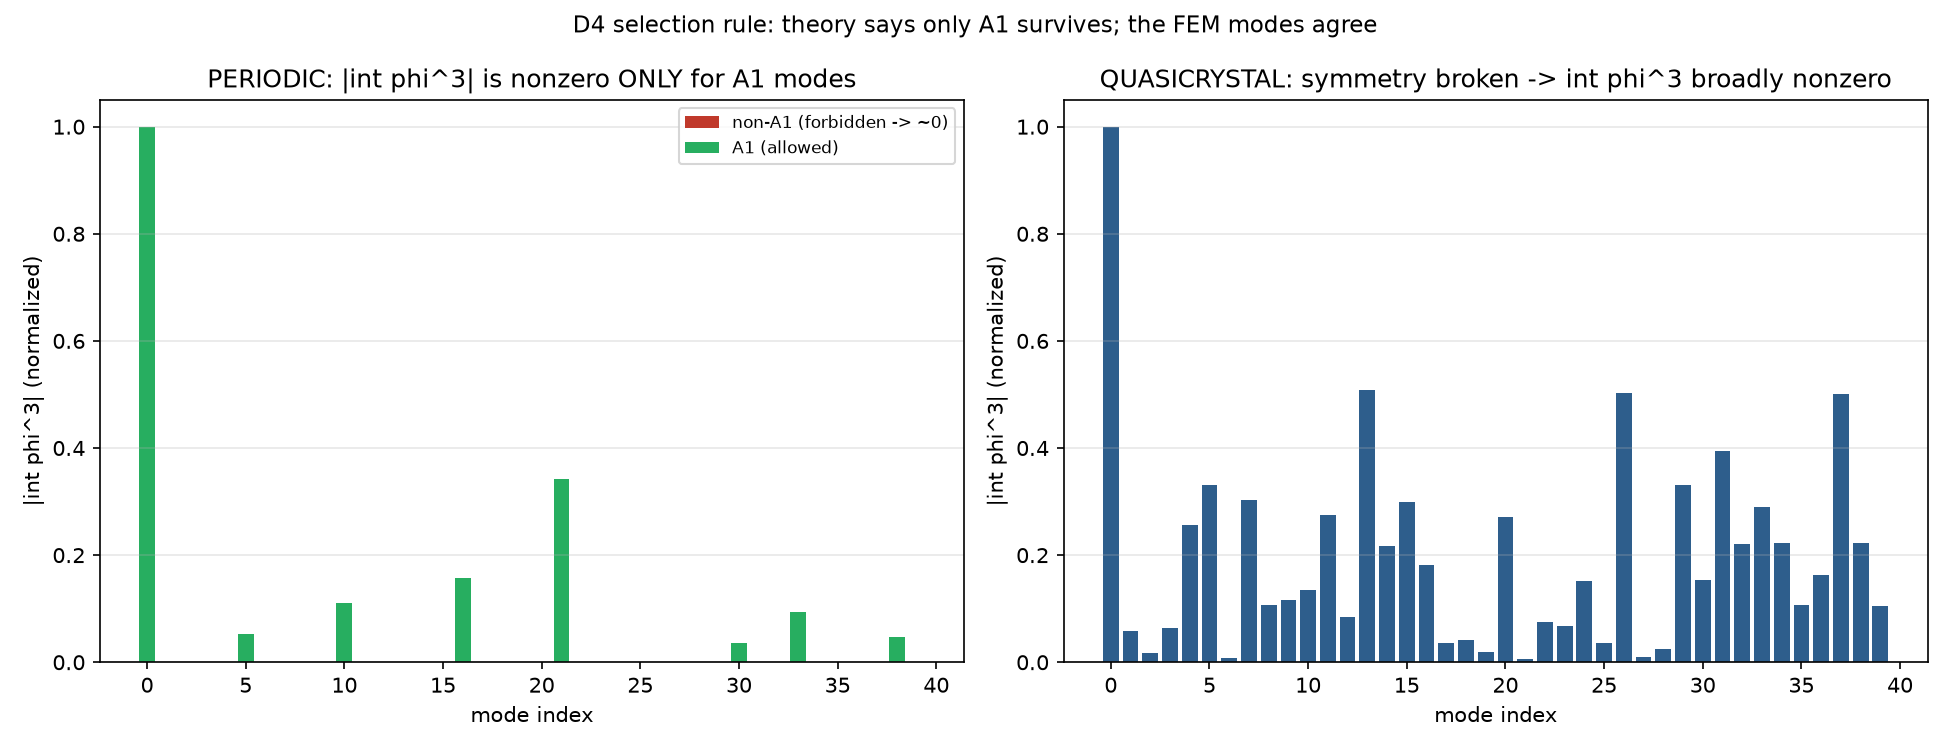
\includegraphics[width=\columnwidth]{verify_selection_rule.png}
\caption{The selection rule on real finite-element modes. \emph{Left:} for the
$D_4$-symmetric plate, $|\int\phi^3|$ is nonzero only for $A_1$ modes (green)
and zero to machine precision for all others (red). \emph{Right:} breaking the
symmetry (quasicrystal) makes $\int\phi^3$ broadly nonzero.}
\label{fig:rule}
\end{figure}

\section{Computing consequence: real, robust, and bounded}

\paragraph{Even/odd fingerprint.}
Equation~\eqref{eq:rule} predicts a sharp signature: a symmetry-broken
substrate should outperform a symmetric one on \emph{even-order} tasks and tie
on \emph{odd-order} ones. It does. Across five even-order tasks (products and
squares of delayed inputs) the quasicrystal wins every one; across five
odd-order tasks (linear and cubic functions) it ties every one, the even-order
gaps exceeding the odd-order ones by one to two orders of magnitude
(Fig.~\ref{fig:dichotomy}).

\begin{figure}[t]
\centering
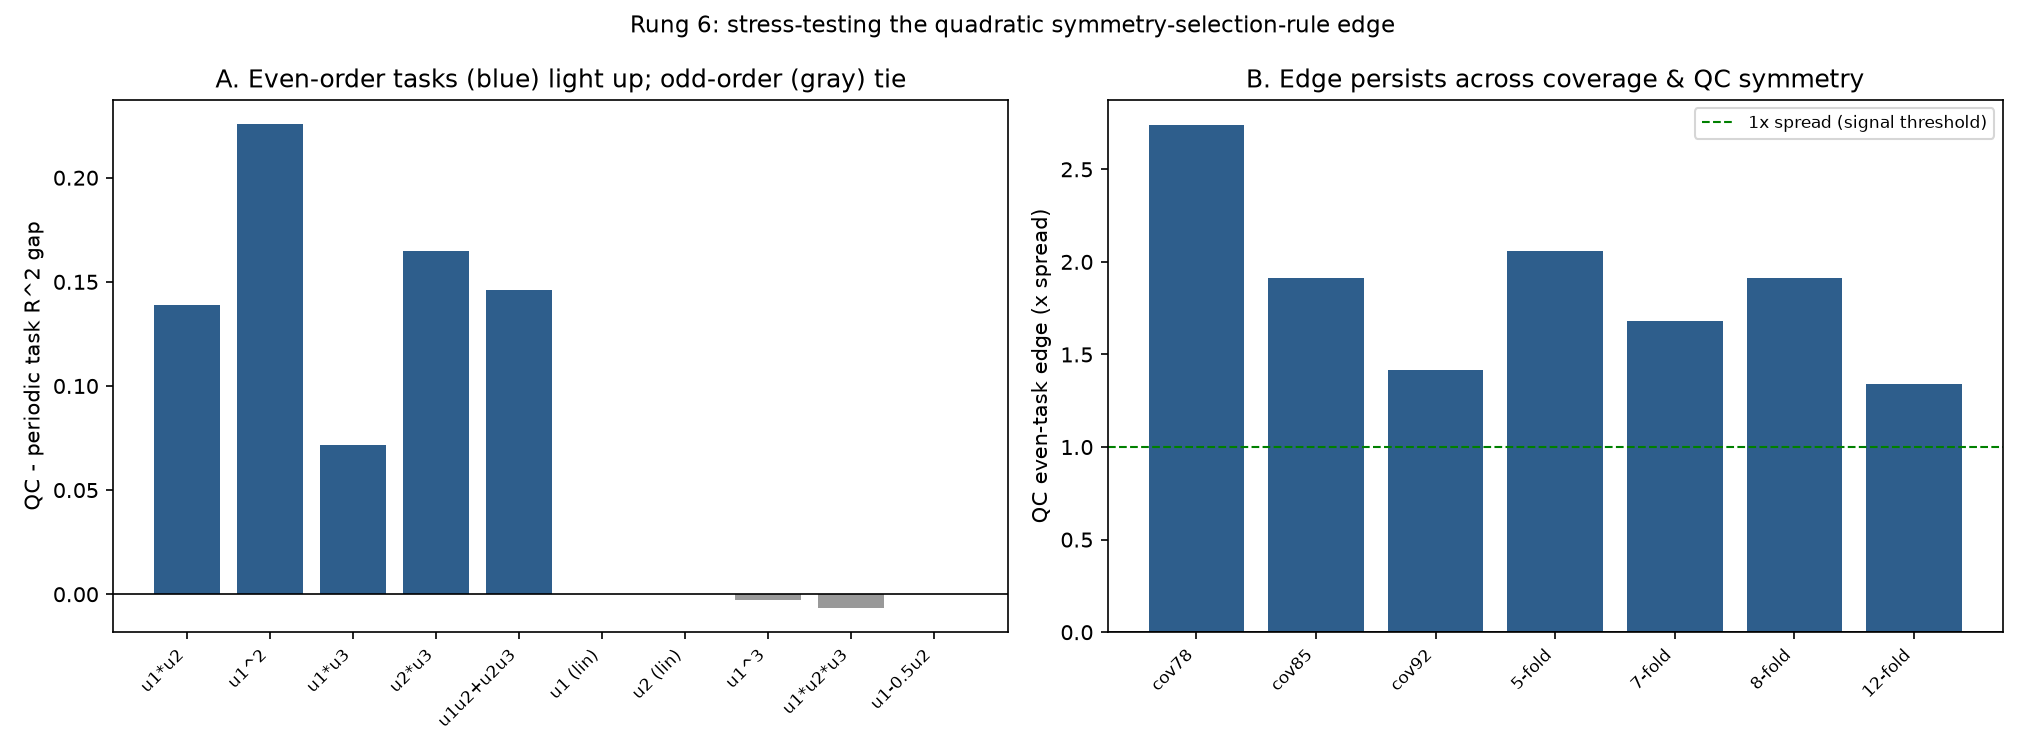
\includegraphics[width=\columnwidth]{reservoir_rung6_stresstest.png}
\caption{\emph{Left:} the symmetry-broken substrate's advantage appears on
even-order tasks (blue) and vanishes on odd-order tasks (gray)---the fingerprint
of the $\int\phi^3$ selection rule. \emph{Right:} the even-order edge persists
across hole coverage and across quasicrystal symmetry order.}
\label{fig:dichotomy}
\end{figure}

\paragraph{Statistical robustness.}
On the product task in the uncoupled regime, cross-validated over five input
realizations and eight actuator positions (40 paired samples, blocked $k$-fold
CV), the advantage is unambiguous: mean $R^2$ gap $+0.184$, $95\%$ confidence
interval $[+0.154,+0.217]$, paired $t$-test $p\approx10^{-13}$, with the
symmetry-broken substrate superior in $100\%$ of pairs. The effect is not a
feature-amplitude artifact: standardizing all readout features leaves it intact
($+0.148$, $p\approx10^{-21}$), confirming that a symmetry-silenced mode is
product-blind at any scale. It is robust across five decades of ridge
regularization.

\paragraph{Symmetry, not aperiodicity.}
The advantage is governed by the \emph{degree of symmetry breaking}, quantified
by the silenced fraction, not by aperiodicity. Across the three substrates the
product-task performance increases monotonically as the silenced fraction
falls (Table~\ref{tab:three}). A \emph{periodic} but low-symmetry plate
captures roughly half of the quasicrystal's advantage over the $D_4$ grid; the
quasicrystal, as the maximal symmetry breaker, captures the most. The operative
principle is therefore the breaking of point symmetry, with the quasicrystal as
one extremal realization rather than a special case.

\begin{table}[t]
\caption{Product-task performance tracks the symmetry-silenced fraction, not
periodicity. Uncoupled regime, cross-validated.}
\label{tab:three}
\begin{ruledtabular}
\begin{tabular}{lcc}
substrate & silenced fraction & product-task $R^2$ \\
\colrule
periodic ($D_4$)        & $0.88$ & $0.273$ \\
periodic (low symmetry) & $0.72$ & $0.362$ \\
quasicrystal (8-fold)   & $0.38$ & $0.457$ \\
\end{tabular}
\end{ruledtabular}
\end{table}

\paragraph{Symmetry from the container, not only the perforation.}
Because the rule depends on the point group of the whole system, the symmetry
can equally be broken by the cavity \emph{boundary}. We confirm this with an
ordinary periodic hole array in cavities of decreasing symmetry: a square
($D_4$) cavity, a rectangular ($C_{2v}$) cavity, and a sheared parallelogram
($C_2$) cavity. The silenced fraction tracks the cavity point group
($0.88,\,0.80,\,0.57$ respectively), and the parallelogram cavity---still a
periodic plate---recovers the full even-order edge, matching the quasicrystal
($R^2=0.50$ vs.\ $0.51$ under identical cross-validation; $p\approx10^{-11}$).
The edge is the same selection-rule mechanism: equalizing $c^{(2)}_i$ across
modes collapses it ($+0.142\to+0.025$), ruling out any artifact of the sheared
mesh, and it is robust across coverage and shear. Mild symmetry reduction (the
rectangle) yields only a faint edge; one must break the mirror planes (the
shear) to recover the full effect. Thus the container shape is itself a
symmetry-breaking design knob, and a low-symmetry \emph{periodic} cavity
suffices---further evidence that the operative variable is point symmetry, not
aperiodicity.

\section{Scope and limitations}

We state the limits plainly, as they bound any application. First, the benefit
is a \emph{shallow}-memory effect. On pure even-order products $u[n-1]u[n-d]$
the absolute performance of \emph{both} substrates collapses with depth---from
$R^2\!\approx\!0.5$ at $d=2$ to $\approx\!0$ by $d=5$ and negative by
$d=9$---because the weakly coupled reservoir cannot hold and multiply
well-separated delays (Fig.~\ref{fig:depth}). The symmetry advantage is real
only where the task is feasible at all. Second, on the NARMA-10 benchmark the
two substrates \emph{tie} ($R^2=0.327$ vs.\ $0.314$): NARMA-10's even-order
term acts at lag~9, where neither substrate succeeds, and its variance is
dominated by linear recurrent memory that both handle equally. Third, there is
an intrinsic tension: the advantage lives in the weakly coupled, low-effective-
dimension regime, whereas deep tasks demand the dimensionality that only strong
coupling supplies---and coupling erases the advantage. The effect is thus an
exact symmetry phenomenon with a modest, sharply circumscribed computational
reach.

\begin{figure}[t]
\centering
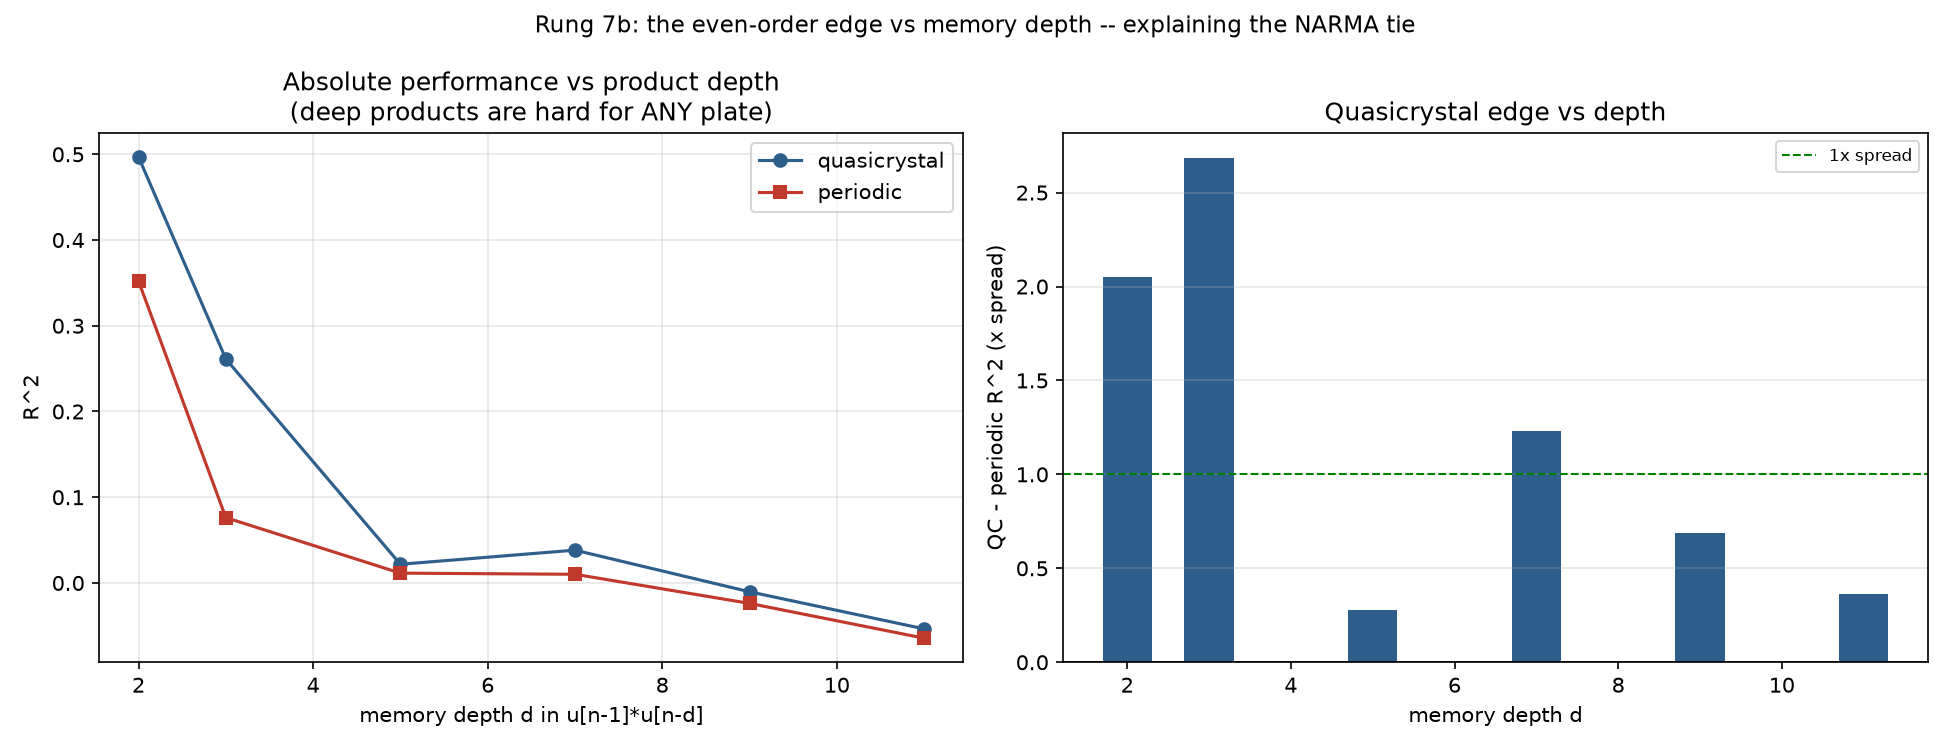
\includegraphics[width=\columnwidth]{reservoir_rung7b_depth.png}
\caption{The even-order advantage is shallow. \emph{Left:} absolute product
performance collapses with delay depth for both substrates. \emph{Right:} the
symmetry advantage is significant only at small depth, where the task is
feasible; this explains the NARMA-10 tie.}
\label{fig:depth}
\end{figure}

\section{Discussion}

Two conclusions follow. The first is cautionary: the geometric richness of
quasicrystalline substrates, often invoked as a reason to expect superior
physical computation, is in our model computationally inert. Spectral
non-degeneracy and dense nonlinear coupling did not help on any task at any
operating point. The second is constructive and exact. The substrate's point
symmetry imposes a selection rule on which nonlinear computations its modes can
perform: a symmetric substrate is blind to even-order computation in all but
its totally symmetric modes, and breaking the symmetry activates it. Nothing in
the derivation is specific to plates or to MEMS; it requires only a modal
physical reservoir, an even-order nonlinearity whose modal strength is
$\int\phi^3$, and a point group. The same rule should therefore constrain
photonic-cavity, spin-wave, mechanical-metamaterial, and electronic-resonator
reservoirs.

As a design heuristic the principle is compact: to obtain even-order
processing from a modal physical computer, break the substrate's point
symmetry; the benefit grows with the fraction of modes thereby de-silenced. A
quasicrystal accomplishes this maximally and ``for free,'' but so, partially,
does any deliberate symmetry reduction of an ordinary periodic design. The
benefit demonstrated here is modest and shallow; whether it can be enlarged---
by even-order transduction engineered for greater modal reach, or by operating
points that reconcile symmetry breaking with higher effective dimension---is
the natural question for future work.

\paragraph{Experimental outlook.}
The selection rule is, above all, directly measurable. Cavity optomechanics
offers a natural test bed: an array of optomechanical cavities with all-optical
readout can map the transverse mode shapes, extract the cubic overlaps
$\int\phi_i^3\,dA$, and verify that they vanish for the symmetry-forbidden
modes and revive when the symmetry is broken---by the perforation or, as shown
here, by the cavity shape. The same optical channels provide independent
per-mode tuning of frequency and damping (the optical-spring and
optomechanical-damping effects), making the silenced fraction itself an
\emph{in situ} control variable rather than a fabrication choice. We caution
that such control reconfigures the linear properties and the readout; it does
not supply the even-order nonlinearity, which must still arise mechanically,
and it does not alter the conserved memory--nonlinearity budget~\cite{dambre2012}
that bounds the computational reach. The value of an optomechanical realization is therefore
as a precise experimental probe of an exact selection rule, not as a route past
the limits identified above.

\section*{Methods}
Finite-element modal analysis uses Mindlin quadrilateral elements with
selective reduced integration and area-fraction homogenization of perforation;
the first $40$ transverse modes are retained and normalized to unit RMS.
Equation~\eqref{eq:modal} is integrated with semi-implicit Euler
($\zeta=0.20$); inputs are i.i.d.\ uniform, with a washout discarded before
training. Readout weights are obtained by ridge regression. Significance is
assessed by paired $t$-test and Wilcoxon signed-rank test over (input seed
$\times$ actuator position) pairs with bootstrap confidence intervals, under
blocked $k$-fold cross-validation with a purge gap to suppress
reservoir-memory leakage. All code and the running findings log are available
in the supplementary repository.

% NOTE: please verify volume/page/year of each reference before final
% submission; they are standard works but double-check the bibliographic details.
\begin{thebibliography}{9}
\bibitem{jaeger2001} H.~Jaeger, ``The `echo state' approach to analysing and
training recurrent neural networks,'' GMD Report 148, German National Research
Center for Information Technology (2001).
\bibitem{maass2002} W.~Maass, T.~Natschl\"ager, and H.~Markram, ``Real-time
computing without stable states: A new framework for neural computation based
on perturbations,'' \emph{Neural Comput.} \textbf{14}, 2531 (2002).
\bibitem{tanaka2019} G.~Tanaka \emph{et al.}, ``Recent advances in physical
reservoir computing: A review,'' \emph{Neural Networks} \textbf{115}, 100 (2019).
\bibitem{appeltant2011} L.~Appeltant \emph{et al.}, ``Information processing
using a single dynamical node as complex system,'' \emph{Nat. Commun.}
\textbf{2}, 468 (2011).
\bibitem{dambre2012} J.~Dambre, D.~Verstraeten, B.~Schrauwen, and S.~Massar,
``Information processing capacity of dynamical systems,'' \emph{Sci. Rep.}
\textbf{2}, 514 (2012).
\bibitem{tinkham1964} M.~Tinkham, \emph{Group Theory and Quantum Mechanics}
(McGraw-Hill, New York, 1964).
\end{thebibliography}

\end{document}
